\hypertarget{words_8c}{
\section{words.c File Reference}
\label{words_8c}\index{words.c@{words.c}}
}
{\tt \#include $<$stdio.h$>$}\par
{\tt \#include $<$stdlib.h$>$}\par
{\tt \#include $<$string.h$>$}\par
{\tt \#include $<$errno.h$>$}\par
{\tt \#include \char`\"{}spat.h\char`\"{}}\par
{\tt \#include \char`\"{}Fasta\-Seq\-IO/fasta\-Seq\-IO.h\char`\"{}}\par


Include dependency graph for words.c:\begin{figure}[H]
\begin{center}
\leavevmode
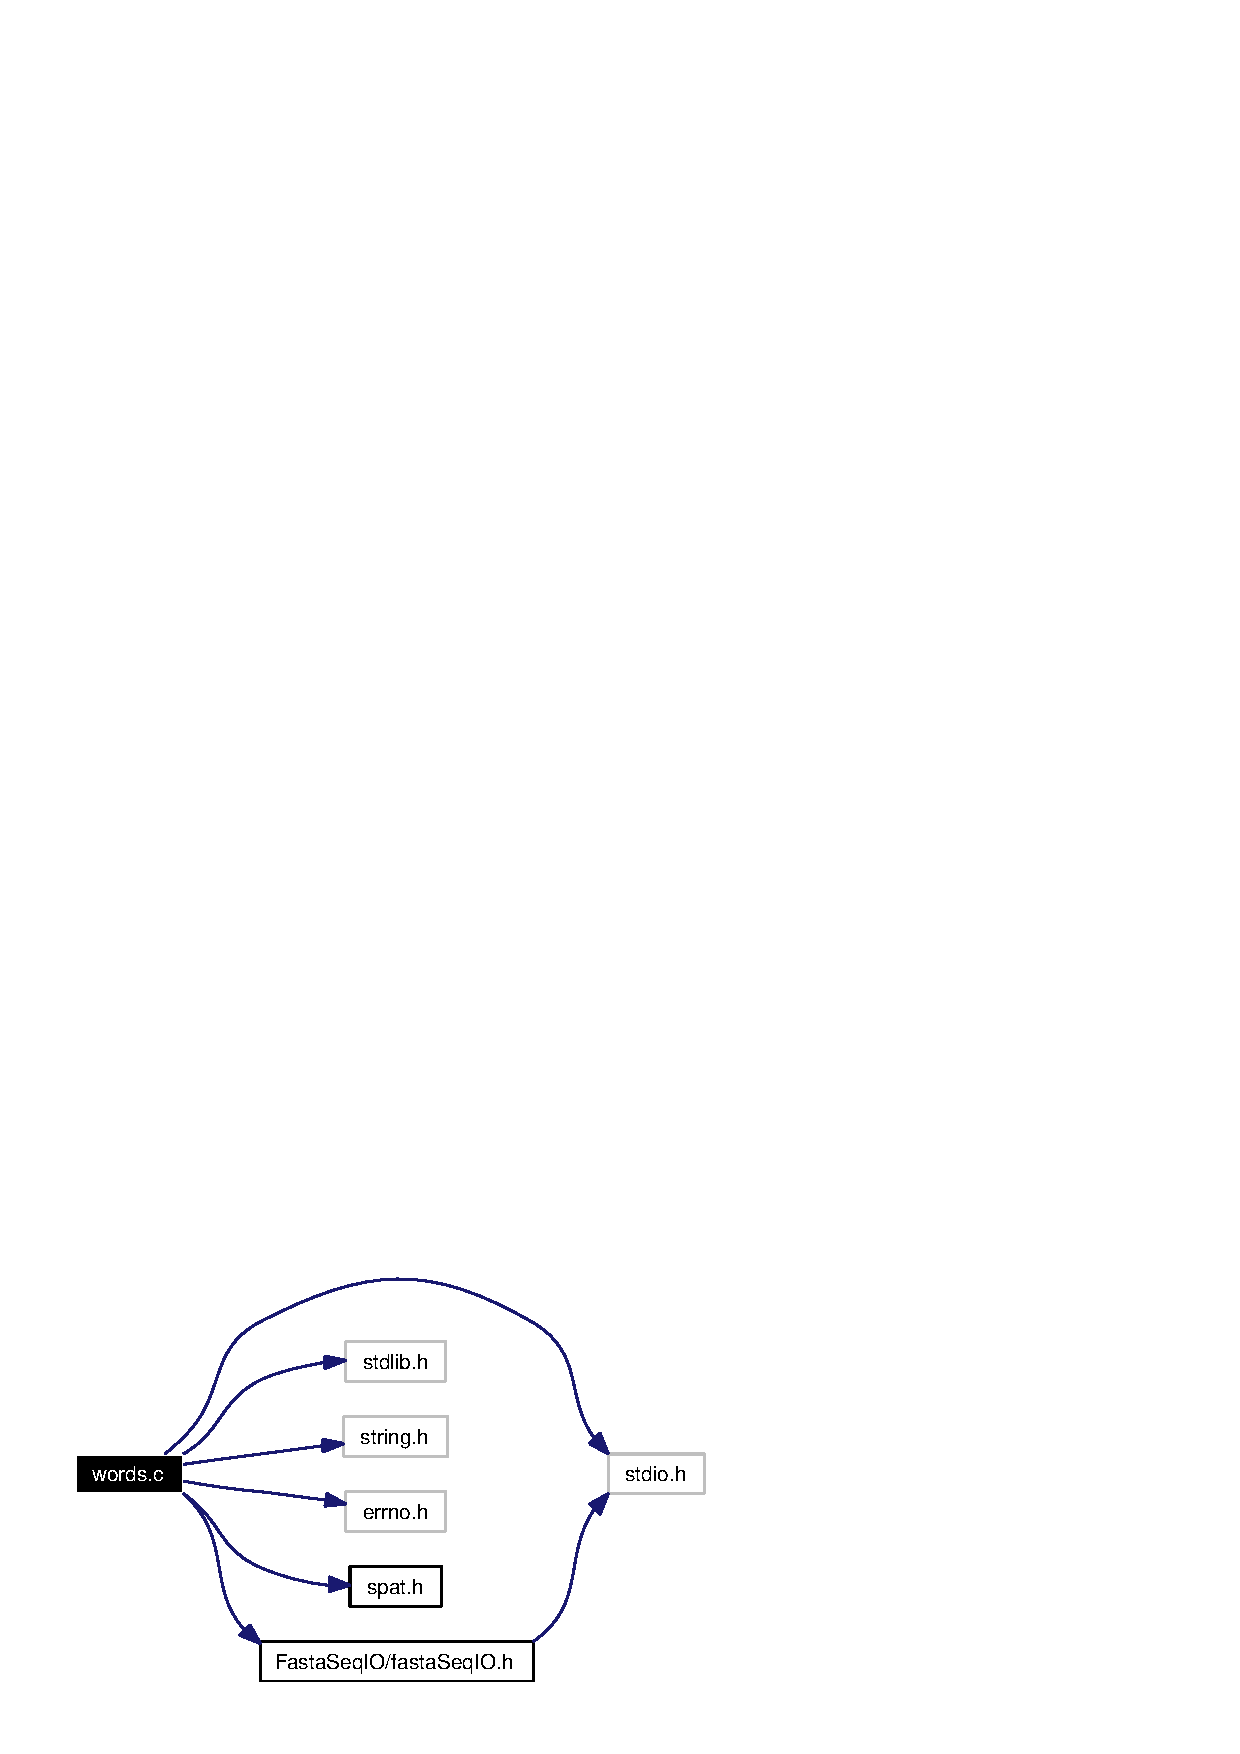
\includegraphics[width=169pt]{words_8c__incl}
\end{center}
\end{figure}
\subsection*{Data Structures}
\begin{CompactItemize}
\item 
struct \hyperlink{structsHashEntry__t}{s\-Hash\-Entry\_\-t}
\item 
struct \hyperlink{structsHash__t}{s\-Hash\_\-t}
\end{CompactItemize}
\subsection*{Defines}
\begin{CompactItemize}
\item 
\#define \hyperlink{words_8c_a0}{SHASH\_\-MAX\_\-KEY\_\-SIZE}~1000
\end{CompactItemize}
\subsection*{Functions}
\begin{CompactItemize}
\item 
int \hyperlink{words_8c_a1}{sieve3} (long n)
\item 
unsigned long \hyperlink{words_8c_a2}{hash1} (unsigned char $\ast$str)
\item 
int \hyperlink{words_8c_a3}{hashpjw} (char $\ast$s)
\item 
\hyperlink{structsHash__t}{s\-Hash\_\-t} \hyperlink{words_8c_a4}{init\-SHash} (int n)
\item 
\hyperlink{structsHashEntry__t}{s\-Hash\-Entry\_\-t} $\ast$ \hyperlink{words_8c_a5}{search\-SHash} (\hyperlink{structsHashEntry__t}{s\-Hash\-Entry\_\-t} $\ast$new\-Entry, \hyperlink{structsHash__t}{s\-Hash\_\-t} $\ast$this\-Hash, int create)
\item 
int \hyperlink{words_8c_a6}{destroy\-SHash} (\hyperlink{structsHash__t}{s\-Hash\_\-t} $\ast$this\-Hash)
\item 
int \hyperlink{words_8c_a7}{print\-SHash} (\hyperlink{structsHash__t}{s\-Hash\_\-t} $\ast$this\-Hash, FILE $\ast$FH)
\item 
int \hyperlink{words_8c_a8}{print\-SPats} (\hyperlink{structsPat__t}{s\-Pat\_\-t} $\ast$a, int n)
\item 
int \hyperlink{words_8c_a9}{destroy\-SPat\-A} (\hyperlink{structsPat__t}{s\-Pat\_\-t} $\ast$words, int wc)
\item 
\hyperlink{structsPat__t}{s\-Pat\_\-t} $\ast$ \hyperlink{words_8c_a10}{count\-Words2} (\hyperlink{structfSeq__t}{f\-Seq\_\-t} $\ast$seq, int num\-Seq, int L, int $\ast$num\-Words)
\end{CompactItemize}


\subsection*{Detailed Description}
This file defines functions that are used in the processing of string based sequences. There are a number of functions defined in this file better used for hashing strings so that the comparison phase can be sped up by only comparing unique words. Heuristically, we have noticed that for sequences in which there is a large degree of redundancy these hashing functions can significantly speed up the comparison phase.

Definition in file \hyperlink{words_8c-source}{words.c}.

\subsection*{Define Documentation}
\hypertarget{words_8c_a0}{
\index{words.c@{words.c}!SHASH_MAX_KEY_SIZE@{SHASH\_\-MAX\_\-KEY\_\-SIZE}}
\index{SHASH_MAX_KEY_SIZE@{SHASH\_\-MAX\_\-KEY\_\-SIZE}!words.c@{words.c}}
\subsubsection[SHASH\_\-MAX\_\-KEY\_\-SIZE]{\setlength{\rightskip}{0pt plus 5cm}\#define SHASH\_\-MAX\_\-KEY\_\-SIZE~1000}}
\label{words_8c_a0}




Definition at line 192 of file words.c.

Referenced by print\-SHash(), and search\-SHash().

\subsection*{Function Documentation}
\hypertarget{words_8c_a10}{
\index{words.c@{words.c}!countWords2@{countWords2}}
\index{countWords2@{countWords2}!words.c@{words.c}}
\subsubsection[countWords2]{\setlength{\rightskip}{0pt plus 5cm}\hyperlink{structsPat__t}{s\-Pat\_\-t}$\ast$ count\-Words2 (\hyperlink{structfSeq__t}{f\-Seq\_\-t} $\ast$ {\em seq}, int {\em num\-Seq}, int {\em L}, int $\ast$ {\em num\-Words})}}
\label{words_8c_a10}


Counts words of size {\em L\/} in the input Fast\-A sequences, hashes all of the words, and returns an array of \hyperlink{structsPat__t}{s\-Pat\_\-t} objects.

Definition at line 373 of file words.c.

References s\-Hash\-Entry\_\-t::data, destroy\-SHash(), s\-Hash\-Entry\_\-t::idx, init\-SHash(), s\-Hash\-Entry\_\-t::key, s\-Hash\-Entry\_\-t::L, s\-Pat\_\-t::length, s\-Offset\_\-t::next, s\-Pat\_\-t::offset, s\-Offset\_\-t::pos, s\-Offset\_\-t::prev, search\-SHash(), s\-Offset\_\-t::seq, sieve3(), s\-Pat\_\-t::string, and s\-Pat\_\-t::support.

Referenced by main().

\scriptsize\begin{verbatim}374 {
375   int i, j;
376   int totalChars = 0;
377   int hashSize;
378   sHashEntry_t newEntry;
379   sHashEntry_t *ep;
380   sHash_t wordHash;
381   sPat_t *words = NULL;
382   int wc = 0;
383   int prev = -1;
384   int l;
385 
386 
387   // Count the total number of characters.  This
388   // is the upper limit on how many words we can have
389   for (i = 0; i < numSeq; i++)
390     {
391       totalChars += strlen (seq[i].seq);
392     }
393 
394   // Get a prime number for the size of the hash table
395   hashSize = sieve3 ((long) (2 * totalChars));
396   wordHash = initSHash (hashSize);
397 
398   // Chop up each sequence and hash out the words of size L
399   for (i = 0; i < numSeq; i++)
400     {
401       prev = -1;
402 
403       // skip sequences that are too short to have
404       // a pattern
405       if (strlen (seq[i].seq) < L)
406     {
407       continue;
408     }
409       for (j = 0; j < strlen (seq[i].seq) - L + 1; j++)
410     {
411 
412       // Make a hash table entry for this word
413       newEntry.key = &(seq[i].seq[j]);
414       newEntry.data = 1;
415       newEntry.idx = wc;
416       newEntry.L = L;
417 
418       // Check to see if it's already in the hash table
419       ep = searchSHash (&newEntry, &wordHash, 0);
420       if (ep == NULL)
421         {
422 
423           // If it's not, create an entry for it
424           ep = searchSHash (&newEntry, &wordHash, 1);
425 
426           // Increase the size of our word array
427           words = (sPat_t *) realloc (words, (wc + 1) * sizeof (sPat_t));
428           if (words == NULL)
429         {
430           fprintf (stderr, "Error!\n");
431           fflush (stderr);
432         }
433           // Add the new word
434           words[wc].string = &(seq[i].seq[j]);
435           words[wc].length = L;
436           words[wc].support = 1;
437           words[wc].offset =
438         (sOffset_t *) malloc (1 * sizeof (sOffset_t));
439           if (words[wc].offset == NULL)
440         {
441           fprintf (stderr, "\nMemory Error\n%s\n", strerror (errno));
442           fflush (stderr);
443           exit (0);
444         }
445           words[wc].offset[0].seq = i;
446           words[wc].offset[0].pos = j;
447           words[wc].offset[0].prev = prev;
448           words[wc].offset[0].next = -1;
449 
450           if (prev != -1)
451         {
452           words[prev].offset[words[prev].support - 1].next = wc;
453         }
454           prev = wc;
455           wc++;
456 
457         }
458       else
459         {
460 
461           // If it is, increase the count for this word
462           ep->data++;
463 
464           // add a new offset to the word array
465           l = words[ep->idx].support;
466           words[ep->idx].offset =
467         (sOffset_t *) realloc (words[ep->idx].offset,
468                        (l + 1) * sizeof (sOffset_t));
469           words[ep->idx].offset[l].seq = i;
470           words[ep->idx].offset[l].pos = j;
471           words[ep->idx].offset[l].prev = prev;
472           words[ep->idx].offset[l].next = -1;
473 
474           // Update the next/prev
475           if (prev != -1)
476         {
477           words[prev].offset[words[prev].support - 1].next = ep->idx;
478         }
479           prev = ep->idx;
480 
481           // Have to put this down here for cases when we create
482           // a word and it is immeadiately followed by itself!!
483           words[ep->idx].support += 1;
484         }
485     }
486     }
487 
488 
489   destroySHash (&wordHash);
490   *numWords = wc;
491   return words;
492 }
\end{verbatim}
\normalsize 


\hypertarget{words_8c_a6}{
\index{words.c@{words.c}!destroySHash@{destroySHash}}
\index{destroySHash@{destroySHash}!words.c@{words.c}}
\subsubsection[destroySHash]{\setlength{\rightskip}{0pt plus 5cm}int destroy\-SHash (\hyperlink{structsHash__t}{s\-Hash\_\-t} $\ast$ {\em this\-Hash})}}
\label{words_8c_a6}


Destroy a hash table, freeing the memory.

Definition at line 272 of file words.c.

References s\-Hash\_\-t::hash, s\-Hash\_\-t::hash\-Size, and s\-Hash\_\-t::i\-Hash\-Size.

Referenced by count\-Words2().

\scriptsize\begin{verbatim}273 {
274   int i;
275   free (thisHash->iHashSize);
276   free (thisHash->hashSize);
277   for (i = 0; i < thisHash->totalSize; i++)
278     {
279       if (thisHash->hash[i] != NULL)
280     {
281       free (thisHash->hash[i]);
282       thisHash->hash[i] = NULL;
283     }
284     }
285   if (thisHash->hash != NULL)
286     {
287       free (thisHash->hash);
288       thisHash->hash = NULL;
289     }
290   return 0;
291 }
\end{verbatim}
\normalsize 


\hypertarget{words_8c_a9}{
\index{words.c@{words.c}!destroySPatA@{destroySPatA}}
\index{destroySPatA@{destroySPatA}!words.c@{words.c}}
\subsubsection[destroySPatA]{\setlength{\rightskip}{0pt plus 5cm}int destroy\-SPat\-A (\hyperlink{structsPat__t}{s\-Pat\_\-t} $\ast$ {\em words}, int {\em wc})}}
\label{words_8c_a9}


This function is used to free up the memory allocated in an array of \hyperlink{structsPat__t}{s\-Pat\_\-t} space objects. The function returns a null pointer.

Definition at line 352 of file words.c.

References s\-Pat\_\-t::offset.

\scriptsize\begin{verbatim}353 {
354   int i;
355   for (i = 0; i < wc; i++)
356     {
357       if (words[i].offset != NULL)
358     {
359       free (words[i].offset);
360       words[i].offset = NULL;
361     }
362     }
363   free (words);
364   words = NULL;
365   return 0;
366 }
\end{verbatim}
\normalsize 


\hypertarget{words_8c_a2}{
\index{words.c@{words.c}!hash1@{hash1}}
\index{hash1@{hash1}!words.c@{words.c}}
\subsubsection[hash1]{\setlength{\rightskip}{0pt plus 5cm}unsigned long hash1 (unsigned char $\ast$ {\em str})}}
\label{words_8c_a2}


A hashing function that returns an integer, given a pointer to a null characterterminated string.

Definition at line 73 of file words.c.

Referenced by search\-SHash().

\scriptsize\begin{verbatim}74 {
75   unsigned long hash = 5381;
76   int c;
77 
78   while ((c = *str++))
79     hash = ((hash << 5) + hash) + c;    /* hash * 33 + c */
80 
81   return hash;
82 }
\end{verbatim}
\normalsize 


\hypertarget{words_8c_a3}{
\index{words.c@{words.c}!hashpjw@{hashpjw}}
\index{hashpjw@{hashpjw}!words.c@{words.c}}
\subsubsection[hashpjw]{\setlength{\rightskip}{0pt plus 5cm}int hashpjw (char $\ast$ {\em s})}}
\label{words_8c_a3}


A hashing function that returns an integer, given a pointer to a null characterterminated string.

Definition at line 89 of file words.c.

\scriptsize\begin{verbatim}90 {
91   char *p;
92   unsigned int h, g;
93 
94   h = 0;
95   for (p = s; *p != '\0'; p++)
96     {
97       h = (h << 4) + *p;
98       if ((g = h & 0xF0000000))
99     {
100       h ^= g >> 24;
101       h ^= g;
102     }
103     }
104   return h;
105 }
\end{verbatim}
\normalsize 


\hypertarget{words_8c_a4}{
\index{words.c@{words.c}!initSHash@{initSHash}}
\index{initSHash@{initSHash}!words.c@{words.c}}
\subsubsection[initSHash]{\setlength{\rightskip}{0pt plus 5cm}\hyperlink{structsHash__t}{s\-Hash\_\-t} init\-SHash (int {\em n})}}
\label{words_8c_a4}


Allocates the memory for a s\-Hash table and initializes some of the elements.

Definition at line 155 of file words.c.

References s\-Hash\_\-t::total\-Size.

Referenced by count\-Words2().

\scriptsize\begin{verbatim}156 {
157   int i = 0;
158   int step = 0;
159   sHash_t this;
160 
161   this.totalSize = n;
162   this.hashSize = (int *) malloc (n * sizeof (int));
163   if (this.hashSize == NULL)
164     {
165       fprintf (stderr, "\nMemory Error\n%s\n", strerror (errno));
166       fflush (stderr);
167       exit (0);
168     }
169   this.iHashSize = (int *) malloc (n * sizeof (int));
170   if (this.iHashSize == NULL)
171     {
172       fprintf (stderr, "\nMemory Error\n%s\n", strerror (errno));
173       fflush (stderr);
174       exit (0);
175     }
176   this.hash = (sHashEntry_t **) malloc (n * sizeof (sHashEntry_t *));
177   if (this.hash == NULL)
178     {
179       fprintf (stderr, "\nMemory Error\n%s\n", strerror (errno));
180       fflush (stderr);
181       exit (0);
182     }
183   for (i = 0; i < n; i++)
184     {
185       this.hash[i] = NULL;
186       this.hashSize[i] = 0;
187       this.iHashSize[i] = step;
188     }
189   return this;
190 }
\end{verbatim}
\normalsize 


\hypertarget{words_8c_a7}{
\index{words.c@{words.c}!printSHash@{printSHash}}
\index{printSHash@{printSHash}!words.c@{words.c}}
\subsubsection[printSHash]{\setlength{\rightskip}{0pt plus 5cm}int print\-SHash (\hyperlink{structsHash__t}{s\-Hash\_\-t} $\ast$ {\em this\-Hash}, FILE $\ast$ {\em FH})}}
\label{words_8c_a7}


This function is used to print the hash out and is generally only used for error checking.

Definition at line 298 of file words.c.

References s\-Hash\-Entry\_\-t::data, s\-Hash\_\-t::hash, s\-Hash\-Entry\_\-t::key, s\-Hash\-Entry\_\-t::L, and SHASH\_\-MAX\_\-KEY\_\-SIZE.

\scriptsize\begin{verbatim}299 {
300   int i, j;
301   char string[SHASH_MAX_KEY_SIZE];
302 
303   for (i = 0; i < thisHash->totalSize; i++)
304     {
305       for (j = 0; j < thisHash->hashSize[i]; j++)
306     {
307 
308       strncpy (string, thisHash->hash[i][j].key, thisHash->hash[i][j].L);
309       string[thisHash->hash[i][j].L] = '\0';
310       fprintf (FH, "%s %d\n", string, thisHash->hash[i][j].data);
311 
312     }
313     }
314   return 0;
315 }
\end{verbatim}
\normalsize 


\hypertarget{words_8c_a8}{
\index{words.c@{words.c}!printSPats@{printSPats}}
\index{printSPats@{printSPats}!words.c@{words.c}}
\subsubsection[printSPats]{\setlength{\rightskip}{0pt plus 5cm}int print\-SPats (\hyperlink{structsPat__t}{s\-Pat\_\-t} $\ast$ {\em a}, int {\em n})}}
\label{words_8c_a8}


This function is used to print out an array of \hyperlink{structsPat__t}{s\-Pat\_\-t} objects and is generally only used for error checking.

Definition at line 321 of file words.c.

References s\-Pat\_\-t::length.

\scriptsize\begin{verbatim}322 {
323   char *s = NULL;
324   int i, j;
325   int size = 0;
326   for (i = 0; i < n; i++)
327     {
328       if (a[i].length > size)
329     {
330       s = (char *) realloc (s, a[i].length * sizeof (char));
331     }
332       strncpy (s, a[i].string, a[i].length);
333       s[a[i].length] = '\0';
334       printf ("%d:  %s\n", i, s);
335       for (j = 0; j < a[i].support; j++)
336     {
337       printf ("\t%d %d -> (%d, %d)\n", a[i].offset[j].seq,
338           a[i].offset[j].pos, a[i].offset[j].prev,
339           a[i].offset[j].next);
340     }
341       printf ("\n");
342     }
343   free (s);
344   return 0;
345 }
\end{verbatim}
\normalsize 


\hypertarget{words_8c_a5}{
\index{words.c@{words.c}!searchSHash@{searchSHash}}
\index{searchSHash@{searchSHash}!words.c@{words.c}}
\subsubsection[searchSHash]{\setlength{\rightskip}{0pt plus 5cm}\hyperlink{structsHashEntry__t}{s\-Hash\-Entry\_\-t}$\ast$ search\-SHash (\hyperlink{structsHashEntry__t}{s\-Hash\-Entry\_\-t} $\ast$ {\em new\-Entry}, \hyperlink{structsHash__t}{s\-Hash\_\-t} $\ast$ {\em this\-Hash}, int {\em create})}}
\label{words_8c_a5}


This function has two purposes. It searches for entries in the hash table and it puts new entries in.

Definition at line 198 of file words.c.

References s\-Hash\_\-t::hash, hash1(), s\-Hash\_\-t::hash\-Size, s\-Hash\_\-t::i\-Hash\-Size, s\-Hash\-Entry\_\-t::key, s\-Hash\-Entry\_\-t::L, SHASH\_\-MAX\_\-KEY\_\-SIZE, and s\-Hash\_\-t::total\-Size.

Referenced by count\-Words2().

\scriptsize\begin{verbatim}199 {
200   char string[SHASH_MAX_KEY_SIZE];
201   unsigned long (*hashFunction) () = &hash1;
202   int i, thisIndex;
203   int status = 0;
204 
205   // A string to store the key
206   strncpy (string, newEntry->key, newEntry->L);
207   string[newEntry->L] = '\0';
208 
209   // The index that this key hashes to
210   thisIndex = hashFunction ((unsigned char *) string) % thisHash->totalSize;
211 
212   // For each member that has this index, check to see
213   // if the key is the same
214   for (i = 0; i < thisHash->hashSize[thisIndex]; i++)
215     {
216       if (strncmp (thisHash->hash[thisIndex][i].key, string, newEntry->L) ==
217       0)
218     {
219 
220       // We found a match
221       /*
222          printf("\t%s already in hash table!\n"); 
223        */
224       status = 1;
225       return &(thisHash->hash[thisIndex][i]);
226       break;
227 
228     }
229     }
230 
231   // If we didn't find the key and we're told to create it,
232   // then allocate new memory for the hashEntry and put it in
233   if (status == 0 && create != 0)
234     {
235 
236       // Allocate space for the new entry at this index
237       if (thisHash->iHashSize[thisIndex] == 0)
238     {
239       thisHash->hash[thisIndex] =
240         (sHashEntry_t *) malloc (sizeof (sHashEntry_t));
241     }
242       else
243     {
244       thisHash->hash[thisIndex] =
245         (sHashEntry_t *) realloc (thisHash->hash[thisIndex],
246                       (thisHash->iHashSize[thisIndex] +
247                        1) * sizeof (sHashEntry_t));
248     }
249       if (thisHash->hash[thisIndex] == NULL)
250     {
251       fprintf (stderr, "\nMemory Error\n%s\n", strerror (errno));
252       fflush (stderr);
253       exit (0);
254     }
255       // Increase our record of the size
256       i = thisHash->hashSize[thisIndex];
257       thisHash->hash[thisIndex][i] = *newEntry;
258       thisHash->iHashSize[thisIndex]++;
259       thisHash->hashSize[thisIndex]++;
260 
261 
262       // Return a pointer to this entry
263       return &(thisHash->hash[thisIndex][i]);
264     }
265   return NULL;
266 }
\end{verbatim}
\normalsize 


\hypertarget{words_8c_a1}{
\index{words.c@{words.c}!sieve3@{sieve3}}
\index{sieve3@{sieve3}!words.c@{words.c}}
\subsubsection[sieve3]{\setlength{\rightskip}{0pt plus 5cm}int sieve3 (long {\em n})}}
\label{words_8c_a1}


Prime number generator: returns first prime number equal or less than\begin{Desc}
\item[Parameters:]
\begin{description}
\item[{\em n.}]\end{description}
\end{Desc}


Definition at line 27 of file words.c.

Referenced by count\-Words2().

\scriptsize\begin{verbatim}28 {
29   int i, p, j;
30   int *a;
31   a = (int *) malloc ((n + 1) * sizeof (int));
32   if (a == NULL)
33     {
34       fprintf (stderr, "\nMemory Error\n%s\n", strerror (errno));
35       fflush (stderr);
36       exit (0);
37     }
38   a[0] = 0;
39   a[1] = 0;
40   for (i = 2; i < n; i++)
41     {
42       a[i] = 1;
43     }
44   p = 2;
45   do
46     {
47       j = 2 * p;
48       do
49     {
50       a[j] = 0;
51       j = j + p;
52     }
53       while (j <= n);
54       p = p + 1;
55     }
56   while (p * p < 2 * n);
57   for (i = n; i > 2; i--)
58     {
59       if (a[i])
60     {
61       free (a);
62       return i;
63     }
64     }
65   free (a);
66   return 0;
67 }
\end{verbatim}
\normalsize 


